\ChapterTitle{生物学}

Avali 是来自 Avalon 卫星的智慧外星生物，拥有高度发达的科技。
它们的外貌与地球白垩纪的恐爪龙非常相似，全身覆盖羽毛，双足直立行走，拥有独特的大眼睛、四只类似兔子的耳朵和长有三根灵巧指爪的双翼，能够操控物体，平均体重约为27-31公斤。
乍一看它们外表温顺，对人类并无威胁。但在 Avalon 卫星上，它们进化成了优秀的飞行者。
尽管拥有发达的大脑和飞行能力，但由于 Avalon 卫星寒冷的自然环境，Avali 的新陈代谢速度远低于人类。

\SubSectionTitle{体型}

与人类相比，Avali 的体型相对较小。
无论性别，成年 Avali 的平均身高在100-120厘米之间。从头到尾尖，Avali 的长度约为120-150厘米。尽管 Avali 的体形较小，但它们进化成了在它们家园食物链顶端的“超级掠食者”。
它们在陆地和空中都拥有强大的能力，强壮的双腿、发达的翅膀、卓越的认知能力和群体战术使它们在家园中独占鳌头，双腿进化得既灵活又能快速奔跑。
脚上的利爪使得它们能够快速穿行于树叶间，攀爬自如。这也赋予了它们良好的负重能力。
Avali 利用这一优势，在树林中狩猎和采集，并将食物带回巢穴。

\begin{wrapfigure}{r}{0.4\textwidth}
	\vspace{-3em}
	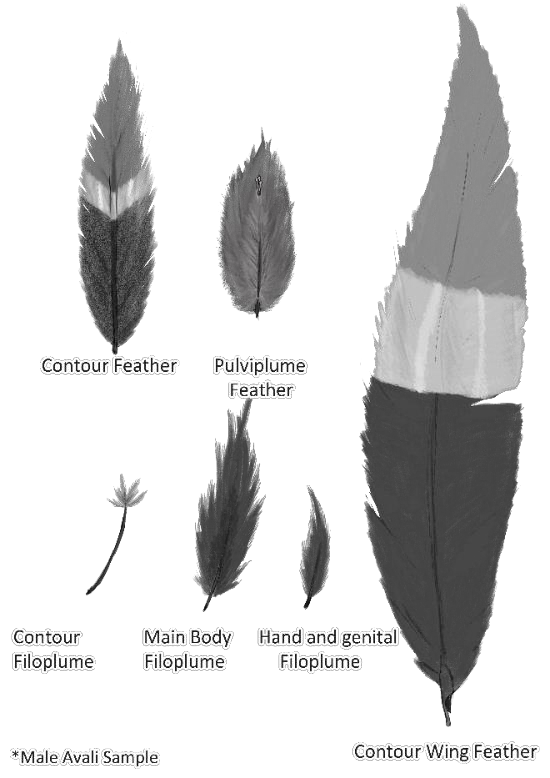
\includegraphics[width=0.4\textwidth]{chapters/chapter1/BIOLOGY/assets/Feathers/Feather_Examples.png}
	\caption{羽毛示例}
	\vspace{-3em}
\end{wrapfigure}

飞行是最常见的出行方式之一，Avali 以强大的飞行能力和在稠密空气中辨别方位的能力而闻名于母星，在其他星球上，他们的翅膀功能有所减弱，但仍能进行低空滑翔和减缓下落速度。
城市和狩猎场的设计充分考虑了 Avali 的飞行需求。然而，大多数货物仍然依靠无人机或人工操控的载具在陆地、海洋和空中运输。
Avali 更依赖无人机和载具来穿越这些环境。

\SubSectionTitle{羽毛}

像地球上的鸟类或其他鸟形类动物一样，Avali 也有一系列特殊的羽毛。
身体的上部和外部覆盖着轮廓型羽毛，这些羽毛表面光滑，自然分泌油脂，以防止积雪。
油腺位于头顶、腋下和骨盆上方。在休息时，Avali 通常会轻抚头部、手臂和骨盆，将油脂涂抹到羽毛上。
一些群体活动中也包括摩擦和梳理外部羽毛，这些活动有助于去除自然脱落的羽毛。

较长的轮廓羽，例如翅膀和冠部的羽毛，其根部血管非常的丰富。
如果这些羽毛被强行拔除，会大量出血。以这种方式脱落的羽毛将在几周后重新长出。

身体下侧和内侧覆盖着较轻且更蓬松的羽毛，有助于身体隔热保暖。
这些特殊的羽毛叫“粉䎃”，是一种能够不断再生的特殊绒毛。它们外层的羽小枝会断裂为粉末，为其他绒毛上油、扑粉，使其保持洁净。

\begin{wrapfigure}{l}{0.4\textwidth}
	\vspace{-1em}
	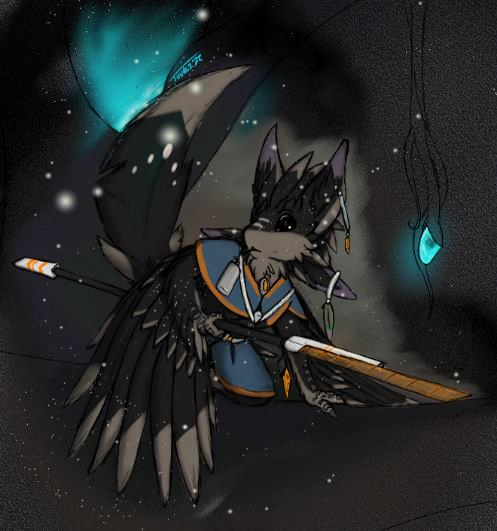
\includegraphics[width=0.4\textwidth]{chapters/chapter1/BIOLOGY/assets/Feathers/Huntress_Avali.png}
	\caption{女猎手 Avali}
	\vspace{-1em}
\end{wrapfigure}

那些较大的轮廓羽毛对热定型反应良好，能形成近乎永久的新造型。
这是一种常见的个性化造型方式。值得注意的是，它们头顶上的冠羽就常被用于此目的，从而形成独一无二的外观。

Avali 的吻部尖端长有一组更细密且带有倒钩的羽毛。
这些独特的羽毛是为了让热量能够传递到吻部的皮肤上，主要用于感知卵的温度。
这些羽毛与相邻的轮廓羽毛一样光滑，但隔热性较差，因此更容易让温度传递。

Avali 身上长有毛羽，这是一种带有神经末梢的特殊羽毛。某些部位，例如翼指和耳朵，这类羽毛分布更为密集。
毛羽有两种不同的类型，功能相似，但一种比另一种更敏感。
较窄长的毛羽分布于身体的主要部位、翅膀和尾尖。
较宽短且更敏感的毛羽则分布于翼爪、生殖器区域、大腿内侧、尾巴下方、耳朵和面部前部。

它们的颜色相对统一，雌雄个体间仅表现出轻微的性别二态性。对于外来者来说，除了花纹和生殖器之外，它们几乎难以区分。
自然色调包括白色、灰色和石板灰，以及柔和低饱和度的大地色系，例如棕色、绿色和褐色。
雄性 Avali 的特征是身体周围有更明亮、近乎虹彩的色带。
雌性的羽毛颜色暗淡，呈双色，通常带有斑点图案。

Avali 一生中羽毛会不断脱落。根据羽毛种类，新羽毛需要3-6周才能完全长成。脱落的羽毛通常颜色暗淡或有损伤。
生活在家园世界寒冷地区的 Avali，除了正常的持续换羽外，每年还会经历两次持续6-8周的换羽期。

\SubSectionTitle{化学构成}

Avali 本质是碳基生物，进化于一个光线微弱的寒冷星球上。
它们的血液由水和氨混合而成，主要成分是铜而不是铁，比例约为 2:1。这使得它们的血液和肌肉呈现紫色至淡紫色。
为了生存，它们需要在富氧环境中呼吸，且氧气浓度不低于 $18\%$。
此外，Avali 需要生活在寒冷的气候中，其适宜的工作温度范围为 $-35\,^\circ\mathrm{C}$ 至 $2\,^\circ\mathrm{C}$（$-31\,^\circ\mathrm{F}$ 至 $37\,^\circ\mathrm{F}$）。
Avali 的核心体温接近 $-7\,^\circ\mathrm{C}$。

Avali 生活在比地球稠密得多的大气层中，大部分地区的大气层密度是地球的两倍。
这种高密度使得某些化学物质的沸点随之升高，从而允许包括 Avali 在内的生命体得以在该星球上进化。
当 Avali 离开母星时，必须穿着特制的防护服来维持所需的高气压。

尽管来自寒冷的星球，但以他们星球的标准来看，Avali 属于高温物种。
Avalai 是内温动物，这意味着他们会消耗大量的代谢能量来产生热量。这种特性是其在母星上飞行所必需的。
然而，尽管比大多数生物都暖和，他们的代谢过程却很缓慢。
Avali 一天会睡好几次，每次睡眠时间都很短。平均而言，Avali 每天总共会睡7到8个小时。
他们经常成群结队地睡觉，互相取暖以进一步节省能量。
由于代谢率低，Avali 的平均寿命相对于其母星而言，只有200到250年。

\SubSectionTitle{呼吸、循环与免疫系统}

\begin{wrapfigure}{l}{0.3\textwidth}
	\vspace{-4em}
	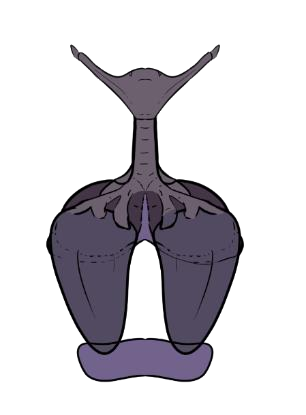
\includegraphics[width=0.3\textwidth]{chapters/chapter1/BIOLOGY/assets/Respiratory_and_Circulation/Respiratory_System.png}
	\caption{呼吸系统}
	\vspace{-1em}
\end{wrapfigure}

Avali 的肺主要由两部分组成：一个较密实的上肺和两个较大的下肺。
上肺主要用于地面活动和休息。空气通过位于后部、耳间和口腔的后气道吸入，或通过这些气道的组合吸入。
空气流经致密的支气管，吸收氧气。一对较大的支气管从上肺延伸至两个较大的下肺。
这些下肺的主要功能是充气，以提高飞行能力，并散发在剧烈运动中产生的热量。
在静息和轻度活动期间，肺部保持微量充气。
相反，在飞行或剧烈运动期间，肺部会持续充满空气，以便更好地吸收氧气。
这些下肺有着许多副支气管，使得 Avali 在飞行过程中能够持续吸收氧气
当这些肺充气时，Avali 的胸部会向外扩张，看起来就像鼓了起来一样。

\begin{wrapfigure}{r}{0.3\textwidth}
	\vspace{-4em}
	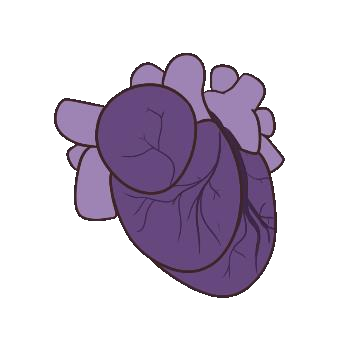
\includegraphics[width=0.3\textwidth]{chapters/chapter1/BIOLOGY/assets/Respiratory_and_Circulation/Avali_Heart.png}
	\vspace{-3em}
	\caption{心脏}

	\vfill

	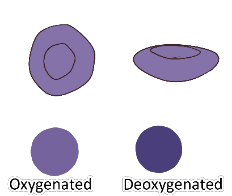
\includegraphics[width=0.3\textwidth]{chapters/chapter1/BIOLOGY/assets/Respiratory_and_Circulation/Blood_cells.png}
	\caption{血细胞}
	\vspace{-1em}
\end{wrapfigure}

Avali 的心脏是四腔心脏，与地球上的心脏类似。
它的血细胞略呈六边形，但仍是圆形的。
心脏有两个较小的上心房，通向两个较大的心室以形成压力。
与鸟类不同，Avali 拥有复杂的肾脏和膀胱，用于排出多余的水分、氨、含氮的废物和其他有害毒素。

Avali 的免疫系统由多种被动防御和一个多级免疫应答系统组成。
在被动免疫方面，Avali 会分泌眼泪、体表开口的黏液、用于口中的唾液以及冲刷泄殖腔的尿液。
被动免疫反应包含一种由 Avali 分泌的广谱抗体，该抗体能够迅速与外来物结合，使得免疫系统能够自动应对威胁。
它们的羽毛和皮肤也能提供抵御外界环境的保护。
当受到抗原（如细菌、真菌和病毒）感染时，多级免疫应答系统会被激活。
初次应答系统由三种免疫细胞组成，它们负责识别、记录和攻击抗原。
这种初级免疫反应主要由巨噬细胞型和中性粒细胞型细胞组成，它们会立即对威胁做出反应。
次级免疫系统则更具攻击性，它由两种类型的活性免疫细胞（A细胞或B细胞）以及C细胞组成。这一阶段还会引起轻微发热和炎症。
三级应答系统负责收集所有残余抗原碎片，并将凋亡和死亡的免疫细胞转运至脾脏。
它们还会持续作用于感染区域，直至15-20天后才结束。

三种活性免疫细胞被归类为A、B和C淋巴细胞。
“A”细胞是主要的攻击细胞。它们识别与抗原结合的钩状抗体分子。
它们攻击并吞噬目标，通过释放酶和蛋白质将其摧毁。
“B”细胞是辅助细胞，它们攻击并附着在真菌、寄生虫等大型抗原上，溶解外部屏障并将其分解，从而协助“A”细胞吞噬这些大型病原体。
“C”细胞是识别与记忆细胞。这些特殊的细胞能够记录潜在威胁，并向免疫应答系统发出信号。
这些细胞附着在异物上，并沉积抗体供其他细胞攻击。
与驻留在 Avali 淋巴结中的其他两种细胞不同，它们始终循环于血液中。

\begin{figure}[htbp]
	\centering
	\begin{minipage}[b]{0.3\textwidth}
		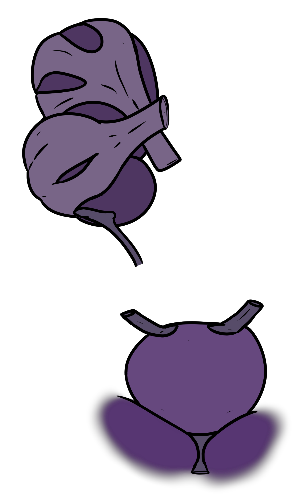
\includegraphics[width=\textwidth]{chapters/chapter1/BIOLOGY/assets/Respiratory_and_Circulation/Avali_Kidney_Bladder.png}
		\caption{肾脏（上图）和膀胱（下图）}
	\end{minipage}
	\begin{minipage}[b]{0.3\textwidth}
		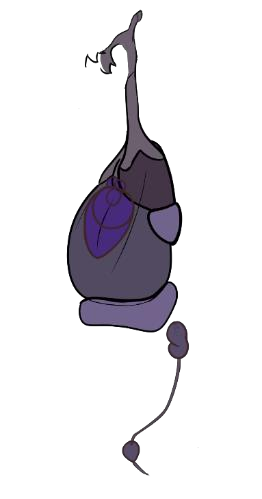
\includegraphics[width=\textwidth]{chapters/chapter1/BIOLOGY/assets/Respiratory_and_Circulation/Avali_Cardiopulmonary_System.png}
		\caption{心肺系统}
	\end{minipage}
	\begin{minipage}[b]{0.3\textwidth}
		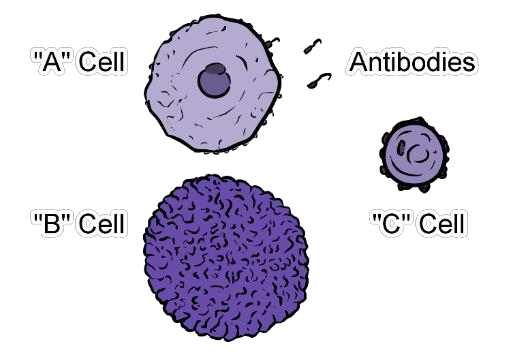
\includegraphics[width=\textwidth]{chapters/chapter1/BIOLOGY/assets/Respiratory_and_Circulation/Avali_Immune_Cells.png}
		\caption{免疫细胞}
	\end{minipage}
\end{figure}

\SubSectionTitle{眼睛}

Avali 的眼睛又大又独特，但与人类相比，他们的视力很差。
他们的眼睛很浅，晶状体非常狭窄。这些结构特征结合起来，使他们能够感知光线，但只能勉强辨认近处的物体。
视力低下是由于其母星光照不足所致，不利于进化出超越基本水平的视觉。
他们的眼睛不像人类的眼睛灵活，只能做一些小动作。
随着 Avali 的进化，他们越来越依赖眼睛来识别和制造工具。
因此，为了弥补进化带来的缺陷，眼睛是 Avali 最常改造强化的部位。

Avali 的眼睛通过位于眼球两侧的两条细小泪腺导管来保持湿润。
这些泪管会分泌氨水泪液，随着眼球运动和眼睑的眨动，这种泪液会扩散到整个眼球。
眼睑边缘的细小倒刺可以阻挡灰尘颗粒。
这些颗粒会被氨水泪液或通过擦拭眼睛的方式清除。
在出现极端天气情况下，Avali 通常会闭上眼睛来保护眼睛免受恶劣天气的影响。

\begin{wrapfigure}{l}{0.35\textwidth}
	\vspace{-2em}
	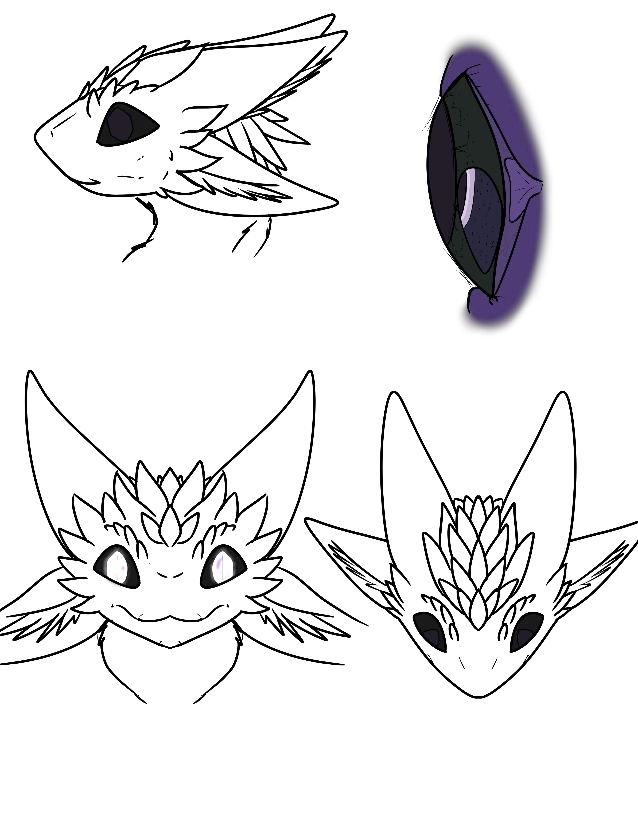
\includegraphics[width=0.35\textwidth]{chapters/chapter1/BIOLOGY/assets/Eyes/Avali_Eyes.png}
	\captionsetup{justification=centering}
	\caption{Avali 的眼睛\\左下角显示的是眼球内部的光线反射。}
	\vspace{-1em}
\end{wrapfigure}

虽然眼睛存在局限，但 Avali 仍能够辨识颜色。
由于到达 Avalon 表面的光线光谱范围有限，它们更侧重于波长在 $590\,\mathrm{nm}$ 至 $1530\,\mathrm{nm}$ 之间的红外光。
能够感知这些光谱使 Avali 能够通过羽毛上特定的自然图案（例如虹彩条纹）轻松区分彼此。
如果没有外部视觉辅助设备，人类会难以清晰地看到这些图案。

对于一般人来说，它们的眼睛主要呈为深灰色或黑色。
它们的眼睛结构与地球生物的眼睛不一样。
角膜完全不透光，在适当光线下会呈现淡紫色。
瞳孔呈狭缝状或八角形，内部完全黑暗。
视网膜上布满了细小的圆形突起，这些突起能够感光并形成彩色图像。
Avali 的眼睛内部有一层反光结构，使其在低光环境下会发出微弱光芒，通常呈现浅灰色。
相应地，这一特性也进一步削弱了眼睛的聚焦能力。

\SubSectionTitle{听觉}

\begin{wrapfigure}{r}{0.35\textwidth}
	\vspace{-2em}
	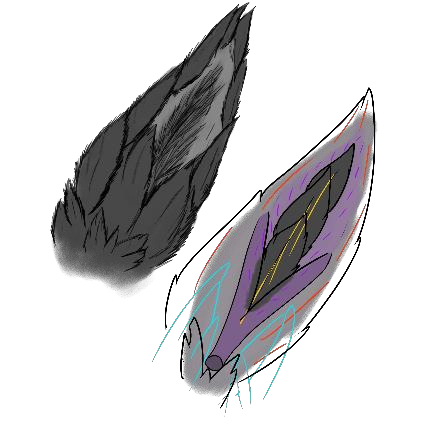
\includegraphics[width=0.35\textwidth]{chapters/chapter1/BIOLOGY/assets/Ears/Avali_Ears.png}
	\caption{Avali 的耳朵}

	\vfill

	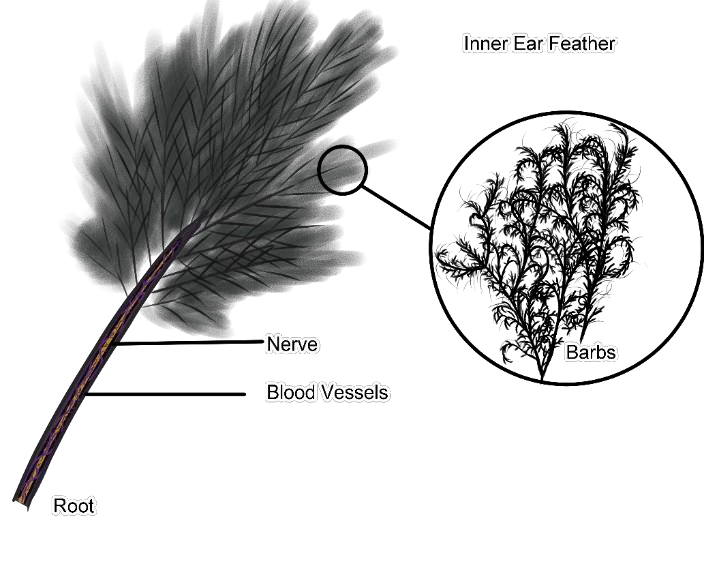
\includegraphics[width=0.35\textwidth]{chapters/chapter1/BIOLOGY/assets/Ears/Avali_Inner_Ear_Feather.png}
	\caption{Avali 的内耳羽毛}

	\vspace{-1em}
\end{wrapfigure}

耳朵是 Avali 最显著的特征。
Avali 有着四只硕大且有关节的耳朵，以及大脑中发达的听觉感觉叶，赋予了他们强大的听觉能力。
头顶上方的两只耳朵可以180度旋转，能够朝前后方。
其自然静止的位置是向后略微朝下。
下方的耳朵虽然不如上方的灵活，但仍能接收到额外的听觉信号。
这些耳朵自然静止时的位置朝向前方，并搭在 Avali 的肩膀上。
每只耳朵都可以单独控制。


Avali 主要依靠听觉。其社会和生活都围绕着听觉展开。
即使在视力完全无法发挥作用的黑暗中，Avali 仍能够通过回声定位来行动与生活。这种能力依赖于它们自身发出的声音，例如呼噜声或轻柔的吱声。
他们耳朵内的特殊羽毛使他们能够感知周围的压力差异，从而获得初步的物体定位能力。
这些羽毛主要用于避免撞到墙壁或从陡峭的地方坠落，它们连接着由血管滋养的长根，并与穿过头骨和大脑的神经相连。
振动通过羽毛的羽枝传递到根部。振动的频率在大脑中进行处理。
这使得 Avali 能够在常规视力无法触及的地方“看到”东西，例如拐角处、洞穴深处，甚至是建筑物的其他楼层。

与大多数动物相比，Avali 的大脑听觉处理中心也更发达。
这使得它们能够专门且独立地处理接收到的听觉信号。
凭借其卓越的听觉进化，Avali 可以听到低至 5Hz、高至 50kHz 的声音。
它们的听觉处理中心能够快速轻松地区分不同的声音，距离测定，甚至提取出特定波长的声音。
Avali 用上耳进行追踪和远距离聆听，下耳则用于近距离聆听和近距离交谈。
它们的耳朵经常会锁定感兴趣的事物，例如聆听对话、音乐、追踪动物等等。
由于具备回声定位功能且听觉系其核心感官，Avali 的双耳对触碰极其敏感

\SubSectionTitle{情绪}

Avali 的表情和肢体语言十分复杂。
头部精细肌肉的发育使它们能够模仿一些与人类相似的表情。
微笑、龇牙咧嘴和皱眉只是它们面部能够表达的几种情绪。
耳朵会配合面部动作移动，以增强情绪的表达。
表达情感最重要的方式是发出声音。
由于听觉是 Avali 的主要感官，它们几乎会为所有情绪发出声音。
Avali 还会调整身体、翅膀和羽毛来进一步表达情感。
某些情绪会使它们炸开羽毛、倾斜身体、调整腿部姿势、展开翅膀或将翅膀收拢。

声音是 Avali 最重要的情感表达方式。
它们会发出各种各样的声音，从简单的啁啾声到咯咯声、类似蛇嘶的嘶嘶声，不一而足。
例如，高亢的啁啾声表示快乐、骄傲和喜悦的情绪。
愤怒、沮丧或嘲讽则会通过第二呼吸道发出嘶嘶声来表达，同时伴随着舌头轻微的咯咯声。
此外，露出牙齿、张开尾巴、裙羽和胸部的羽毛，以及呼出大量空气、呼出大量空气或通过副肺吸气都是愤怒的迹象。
满足、爱、调情和脸红等情绪则会通过咕噜声和低吟来表达。
这些声音通常还会伴随着眼睛下方的羽毛向外张开，这是一种脸红的表现。
在闲暇或好奇时，会发出咔哒声和随意的啁啾声。

\SubSectionTitle{嗅觉}

Avali 用舌头进行“嗅闻”，就像地球上的蛇一样，通过品尝空气来感知气味。
经常可以看到它们不停地品尝周围的空气。
Avali 并没有传统意义上的鼻腔来感知空气中的颗粒，它们的感知受器位于口腔顶部。

细长的嗅球位于大脑底部，靠近口腔顶部。
由于缺乏鼻腔，Avali 的第二呼吸道不在头部前部，而是在颅骨后部的两耳之间，与调节压力的咽鼓管相连。
仔细观察 Avali 的后脑勺，可以看到它们两耳之间的羽毛在呼吸时会扇动。

\clearpage

\begin{figure}[!tp]
	\centering
	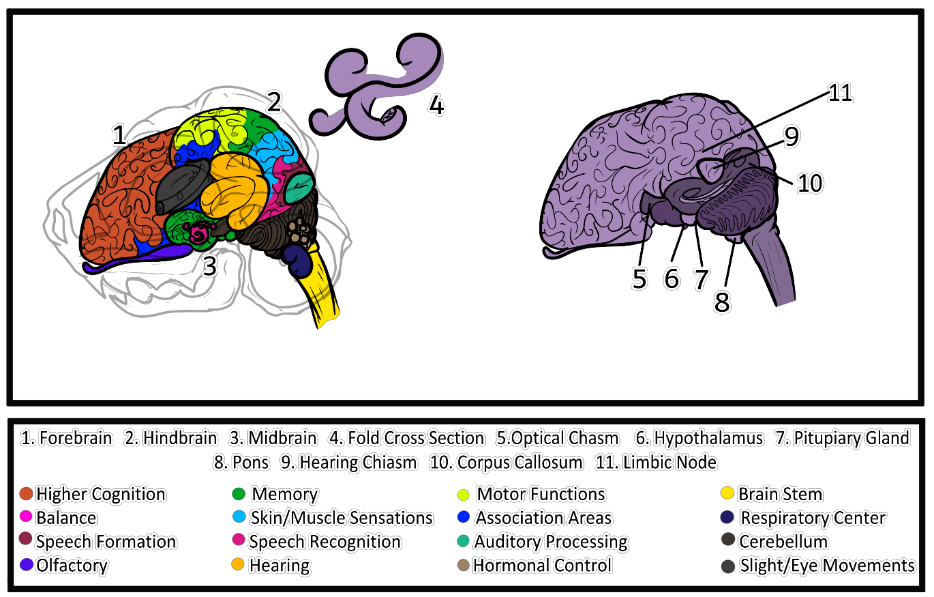
\includegraphics[width=\textwidth]{chapters/chapter1/BIOLOGY/assets/Smelling/Brain_Region_Map.png}
	\caption{Avali 脑部区域图}
\end{figure}

\SubSectionTitle{大脑}

Avali 的大脑体积庞大，具备复杂的思维能力与解决问题的能力。
这种能力使他们成为星球上强大的掠食者，并发展成为先进的太空文明。
他们的大脑结构独特，由分为两半的后脑、中脑以及巨大的前脑组成。
Avali 的大脑向下延伸至头骨的吻部，即推测的鼻腔所在位置。

Avali 的前脑非常显眼，它是从大脑中心延伸出的、不分叶的单一整体，没有明显的“左右两半”之分。
这部分脑区包含了我们今天所知的海马体、高级认知功能区、联想区以及除听觉记忆之外的记忆功能区。
嗅觉通路也位于此处。

大脑中心是中脑。
包含两个较大的听觉处理叶、听觉沟、光感受器（光感受器）、平衡和定向沟、协调反应中心以及下丘脑。
中脑还将分叶的后脑与前脑、小脑、脊髓和延髓连接起来。

后脑由两个半球组成，位于大脑后部。
两半球之间有一条清晰的接缝将其一分为二，使其外观特征十分显著。
大脑的这一区域负责控制本能性动作与精细肌肉运动、听觉记忆、皮肤与肌肉感知、语言的识别与构建，并承担后续的听觉处理工作。

\SubSectionTitle{骨骼结构}

